\chapter{Cos’è TCFS e come funziona} 
TCFS (Transparent cryptografic file system) è un FS crittografico con lo scopo di rendere totalmente trasparente all’utente le operazioni crittografiche sottostanti. Un filesystem crittografico permette all’utente di proteggere i dati rendondoli illegibili ad utenti non autorizzati. Molti FS crittografici richiedono all’utente di eseguire comandi particolari per gestire i file inclusi al loro interno, TCFS evita queste scomodità ed evita di dover ricordare una password per accedere ai contenuti, evitando di compromettere la sicurezza. TCFS sfrutta le funzionalità di FUSE per interporsi nella comunicazione tra userspace e kernel in modo da cifrare e decifrare i contenuti dei file e dei nomi dei file. Questo FS ha lo scopo principale di criptare i dati prima di inviarli su un server remoto, tramite protocolli di rete come NFS o webdav e simili, a patto che supportino gli attributi estesi. In questo modo, TCFS garantisce che i dati siano protetti sia in transito che in riposo, cioè sia durante la comunicazione tra il client e il server, sia quando sono memorizzati sul server. L'architettura di TCFS presuppone che il client sia fidato, ma chiaramente non si fida del server. Un aspetto distintivo, sebbene non primario dell’implementazione di TCFS, basata su FUSE, è la capacità tecnica di cifrare anche file in directory locali. Questo rappresenta un valore aggiunto significativo, poiché estende la protezione dei dati oltre il contesto di rete, garantendo la sicurezza dei dati anche a livello locale. In conclusione, l’approccio adottato da TCFS offre un equilibrio ottimale tra facilità d’uso, versatilità e sicurezza dei dati, rendendolo una soluzione ideale per affrontare le sfide della privacy odierna.

\section{Le differenze tra i filesystem non trasparenti e TCFS}
I filesystem crittografici non trasparenti richiedono che l’utente esegua comandi specifici per gestire i file all’interno del sistema, mentre TCFS (Transparent Cryptographic File System) rende queste operazioni crittografiche completamente trasparenti all’utente. Questa trasparenza offre un equilibrio ottimale tra facilità d’uso, versatilità e sicurezza dei dati.

\subsection{Confronto con CODA}
CODA è un sistema di file distribuito sviluppato presso l’Università di Carnegie Mellon che mira a fornire un sistema di file altamente disponibile e scalabile. A differenza di TCFS, CODA non è progettato specificamente per fornire funzionalità crittografiche, tuttavia, CODA supporta la crittografia per la sicurezza dei dati durante la trasmissione. A differenza di CODA, TCFS assicura che i dati sulla rete e a riposo siano crittografati.
Mentre TCFS si concentra sulla trasparenza delle operazioni crittografiche per l’utente, CODA si concentra sulla fornitura di un sistema di file distribuito robusto e resiliente. CODA utilizza tecniche come la replica dei server e la cache del client per fornire accesso ai file anche quando la rete è instabile o non disponibile.

\subsection{Confronto con AFS}
L’Andrew File System (AFS) è un filesystem distribuito che utilizza un insieme di server fidati per presentare uno spazio dei nomi dei file omogeneo e indipendente dalla posizione a tutte le workstation client. Tuttavia, a differenza di TCFS, AFS non fornisce funzionalità crittografiche trasparenti \cite{AnalisiDiDiversiFS}.

\subsection{Confronto con CFS}
Il Cryptographic File System (CFS) è un altro sistema di file crittografico che fornisce la crittografia a livello di file. A differenza di TCFS, CFS non è progettato per essere completamente trasparente per l’utente. Invece, CFS richiede che l’utente monti esplicitamente il filesystem crittografico e fornisca una chiave di crittografia.
Mentre TCFS si concentra sulla trasparenza delle operazioni crittografiche per l’utente, CFS si concentra sulla sicurezza dei dati. CFS utilizza una chiave di crittografia per crittografare i dati, il che significa che solo gli utenti che conoscono la chiave possono accedere ai dati. In conclusione, sia TCFS che CFS offrono funzionalità uniche e preziose. TCFS si distingue per la sua trasparenza nelle operazioni crittografiche, rendendo facile per gli utenti proteggere i loro dati senza dover gestire direttamente la crittografia. Ambedue offrono un alto livello di sicurezza dei dati, con l’uso di chiavi di crittografia per proteggere l’accesso ai dati, ma TCFS lo fa in maniera trasparente. \cite{AnalisiTCFSeCFS}.

\section{Caratteristiche di TCFS}
TCFS pone come carattiristiche principali:
\begin{itemize}
    \item \textbf{Trasparenza}: TCFS rende la cifratura e la de-cifratura dei file invisibili all’utente, che può usare il filesystem ignaro della complessità sottostante, senza dover inserire password o usare comandi specifici.
    \item \textbf{Sicurezza}: TCFS usa l’algoritmo AES GCM per criptare i file, considerato uno dei più sicuri e diffusi al mondo, usando delle chiavi generate casualmente, in modo da ridurre il rischio di perdita o furto delle chiavi. Inoltre questo algoritmo è spesso utilizzato date le sue ottime performance.
    \item \textbf{Flessibilità}: TCFS si basa su FUSE, una tecnologia che permette di creare e gestire dei filesystem a livello utente, senza dover modificare e ricompilare il kernel del sistema operativo. Questo rende TCFS compatibile con diversi supporti fisici e portabile verso diversi OS Inoltre e permette di personalizzare il filesystem sottostante (riferirsi alla figura \ref{fig:TCFS-flow}) in base alle proprie esigenze. 
\end{itemize}

\section{Funzionamento e architettura di TCFS} 
TCFS è diviso in varie parti, un modulo userspace che si interfaccia con FUSE, un server REST per il threshold sharing e un programma helper che aiuta l'utente ad avviare TCFS. Ogni parte in TCFS è di fatto indipendente dalle altre, di seguito viene illustrata in maggiore dettaglio l'architettura del FS.

\subsection{L'architettura di TCFS e dove si trova nello stack} 
Il modulo TCFS agisce come un intermediario tra l’utente e il modulo kernel di FUSE. Questo posizionamento strategico consente a TCFS di intercettare e gestire le invocazioni dei comandi che operano sui file. Una volta che TCFS ha elaborato le operazioni, le inoltra al kernel, che a sua volta esegue l’operazione corrispondente sul file.

Per illustrare meglio questo processo, consideriamo due esempi comuni: la lettura e la scrittura di un file.
\begin{itemize}
    \item \textbf{Lettura di un file}: Quando un utente tenta di leggere un file, l’invocazione del comando di lettura viene prima intercettata dal modulo kernel  di FUSE (grazie a VFS), che inoltra a TCFS la richiesta di lettura. TCFS quindi decifra il contenuto del file e popola un buffer, preallocato dal modulo kernel, con i dati decifrati. Successivamente vengono restituiti i dati decifrati all’utente.
    \item \textbf{Scrittura di un file}: Analogamente, quando un utente scrive su un file, l’invocazione del comando di scrittura viene intercettata da TCFS, che cifra i dati e inoltra i dati cifrati al modulo kernel di FUSE, che scrive i dati cifrati sul file.
\end{itemize}
In entrambi i casi, TCFS garantisce che i dati siano sempre cifrati quando sono memorizzati sul file, fornendo così una protezione crittografica dei dati. Questo meccanismo di interposizione tra l’utente e il kernel consente a TCFS di fornire un livello aggiuntivo di sicurezza e privacy, proteggendo i dati dell’utente da accessi non autorizzati.
\begin{figure}[H]
    \centering
    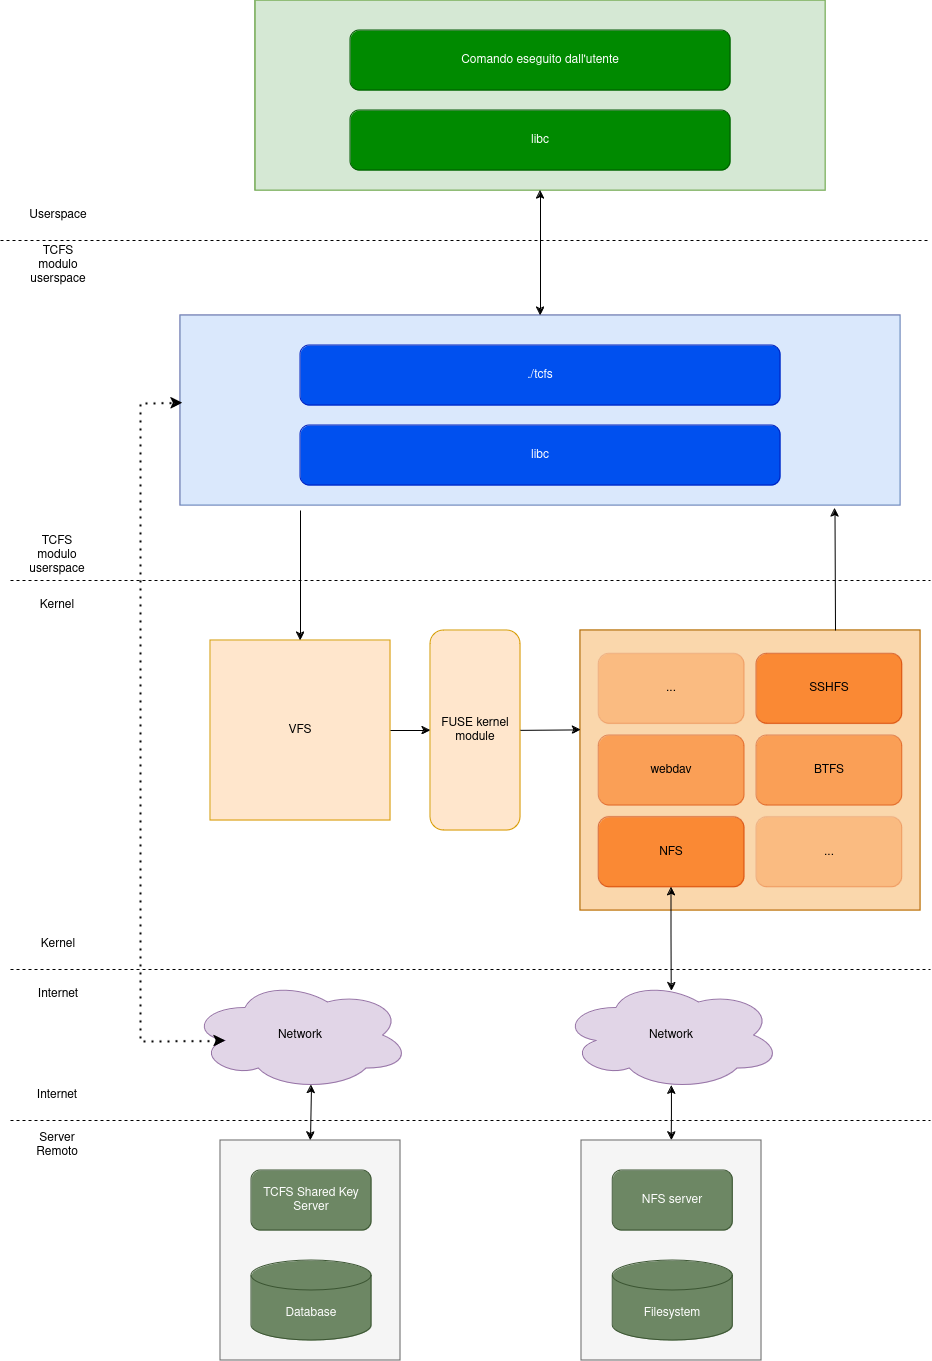
\includegraphics[width=14cm]{capitoli/risorse/TCFSflow.png}
    \caption{Architettura di TCFS}
    \label{fig:TCFS-flow}
\end{figure}

\subsubsection{Chiarimenti su VFS e FUSE}
Il Virtual File System (VFS) è un’interfaccia astratta a livello del kernel del sistema operativo che fornisce un meccanismo per l’interazione uniforme con vari filesystem. Il VFS è responsabile della gestione e coordinamento delle richieste di I/O tra il kernel del sistema operativo e i vari filesystem sottostanti. Esso fornisce un insieme comune di API per le operazioni sui file, indipendentemente dal tipo di filesystem sottostante. Questo livello di astrazione consente al sistema operativo di supportare una vasta gamma di filesystem, come ext4, NTFS, FAT32, ecc., senza dover implementare le specifiche di ciascuno di essi nel kernel.
FUSE (Filesystem in Userspace) è un modulo del kernel che fornisce un’interfaccia per la creazione di filesystem personalizzati in spazio utente. FUSE estende le funzionalità del VFS permettendo agli utenti di implementare un filesystem come un’applicazione a livello di utente, piuttosto che come un modulo del kernel. Questo offre una maggiore flessibilità e sicurezza, poiché gli errori nel codice del filesystem non possono causare crash del sistema.
FUSE si interfaccia con il VFS tramite un’API specifica. Quando un processo effettua una richiesta di I/O su un file o una directory all’interno di un filesystem FUSE, il VFS inoltra la richiesta al modulo FUSE. FUSE a sua volta traduce la richiesta in un formato comprensibile per l’applicazione del filesystem FUSE e la inoltra all’applicazione.
L’applicazione del filesystem FUSE, che è un’applicazione standalone che utilizza la libreria libfuse, implementa la logica specifica del filesystem. Questa applicazione gestisce le richieste provenienti da FUSE, elabora i dati necessari e invia una risposta a FUSE. Ad esempio, se viene richiesta la lettura di un file, l’applicazione del filesystem FUSE leggerà il file dal disco, elaborerà i dati se necessario, e invierà i dati letti a FUSE come risposta.
FUSE quindi restituisce la risposta al VFS, che a sua volta la restituisce al processo che ha effettuato la richiesta originale. In questo modo, FUSE agisce come un ponte tra il VFS a livello di kernel e il filesystem implementato in spazio utente.
In sintesi, il VFS, FUSE e l’applicazione del filesystem FUSE lavorano insieme per fornire un’interfaccia uniforme per la gestione dei filesystem, consentendo al contempo la creazione di filesystem personalizzati in spazio utente. Questo approccio oltre a fornire una grande flessibilità, offre anche un modello di progettazione particolarmente utile, flessibile e semplificato per lo sviluppo di nuovi filesystem, la prototipazione di funzionalità del filesystem e la creazione di filesystem per scopi specifici.

\subsection{Il modulo userspace di TCFS} 
FUSE mette a disposizione una struttura dati che mappa le funzioni specificate da TCFS con le API di FUSE. Nel caso di TCFS le operazioni supportate sono:
\begin{lstlisting}[style=C, caption=Mappa FUSE API alle funzioni di TCFS , label=C-TCFS-FUNCS]
static struct fuse_operations tcfs_oper = {
  .opendir = tcfs_opendir,
  .getattr = tcfs_getattr,
  .access = tcfs_access,
  .readlink = tcfs_readlink,
  .readdir = tcfs_readdir,
  .mknod = tcfs_mknod,
  .mkdir = tcfs_mkdir,
  .symlink = tcfs_symlink,
  .unlink = tcfs_unlink,
  .rmdir = tcfs_rmdir,
  .rename = tcfs_rename,
  .link = tcfs_link,
  .chmod = tcfs_chmod,
  .chown = tcfs_chown,
  .truncate = tcfs_truncate,
  .utimens = tcfs_utimens,
  .open = tcfs_open,
  .read = tcfs_read,
  .write = tcfs_write,
  .statfs = tcfs_statfs,
  .create = tcfs_create,
  .release = tcfs_release,
  .fsync = tcfs_fsync,
  .setxattr = tcfs_setxattr,
  .getxattr = tcfs_getxattr,
  .listxattr = tcfs_listxattr,
  .removexattr = tcfs_removexattr,
};
\end{lstlisting}
Nel contesto di FUSE, quando si parla di funzioni, ci si riferisce alle funzioni di callback che l’utente deve implementare per definire il comportamento del FS. Queste funzioni vengono poi chiamate da FUSE quando si verificano determinate operazioni sul FS, come la lettura di un file o la creazione di una directory.
Ogni funzione di callback ha un insieme specifico di parametri che deve accettare. Questi parametri sono definiti da FUSE e possono includere informazioni come il percorso di un file o la dimensione di un buffer di lettura. Il numero e il tipo di questi parametri sono determinati dalla specifica operazione sul FS che la funzione deve gestire.
Inoltre, FUSE può pre-allocare o pre-riempire alcuni di questi parametri con i dati necessari prima di chiamare la funzione di callback. Ad esempio, se la funzione di callback è responsabile della lettura di un file, FUSE potrebbe pre-allocare un buffer di lettura e passarlo come parametro alla funzione.
In sintesi, FUSE specifica quali parametri una funzione deve accettare e può anche pre-allocare o pre-riempire questi parametri con i dati necessari prima di chiamare la funzione. Questo permette all’utente di concentrarsi sulla logica specifica del FS, senza doversi preoccupare della gestione dei dettagli a basso livello.

\subsection{Il key manager di TCFS} 
TCFS custodisce le chiavi dell'utente all'interno del kernel sfruttando il set di utilities Keyutils, incluso in Linux. Keyutils è un insieme di utility per la gestione e conservazione delle chiavi nel kernel, esso permette di mantenere una chiave all'interno del keyring dell'OS; questa chiave è identificata da in key\_id, che viene specificato nel file di configurazione di TCFS. Il fetch della chiave viene eseguito dall'apposita systemcall keyctl\_read e la chiave viene concessa se e solo se l'ID della chiave è valido e l'utente ha i permessi necessari per richiederla. In generale, l’utente che ha inserito la chiave nel keyring ha i permessi per accedervi, ma può anche concederli o revocarli ad altri utenti, usando il comando keyctl setperm. Chiaramente è necessario ricordare che per definizione dell'architettura di TCFS l'utente è sempre fidato, dunque come abbia ottenuto la chiave non impatta sulla sicurezza del progetto.
Nello specifico è stata sviluppata una libreria denominata key\_utils che espone tre funzioni:
\begin{itemize}
    \item \textbf{char *get\_key ()}:che ottiene la chiave dal kernel e restituisce un buffer contenente la chiave stessa. Il buffer viene allocato dal kernel e condiviso con TCFS.
    \item \textbf{void free\_key (const char *key)}: Che prende in input il puntatore alla chiave, sovrascrive l'area di memoria con "0" e libera lo spazio della chiave.
    \item \textbf{void set\_key\_id(const char *value)}: Che permette di settare l'id della chiave per la sessione attuale di TCFS.
\end{itemize}

\subsection{Il server REST di TCFS} 
Durante il corso del progetto è stato sviluppato un REST in Golang atto a gestire il threshold sharing attraverso l'algoritmo di Shamir. Questo consente di garantire la sicurezza e la riservatezza nell'accesso ai file soggetti al threshold sharing. Si ricorda che questo server non è necessario per il funzionamento di TCFS che ne è di fatti indipendente.
Quando un file viene condiviso utilizzando il threshold sharing la chiave del file viene suddivisa in multiple parti, e ciascuna parte è associata a un share univoco. Il file completo può essere ricostruito solo quando un numero specificato di share viene combinato insieme, rispettando il threshold definito. Non è stato implementato un modo per riottenere la chiave del file.

\subsubsection{Cos'è l'algoritmo di Shamir e come funziona}
Il threshold sharing, ottenuto tramite l'algoritmo di Shamir è un concetto fondamentale nell'ambito della crittografia e della sicurezza informatica. Esso consente di suddividere un segreto in multiple parti, note come "share", in modo che il segreto possa essere ricostruito solo quando un numero minimo di share viene combinato insieme. Questo numero minimo è definito come "threshold". Questa metodologia fornisce un elevato livello di sicurezza, in quanto anche se alcuni share vengono compromessi o ottenuti da parte di terzi non autorizzati, il segreto non può essere ricostruito senza il numero minimo di share richiesto. Pertanto, l'implementazione del threshold sharing tramite l'algoritmo di Shamir nel server REST di TCFS contribuisce in modo significativo alla protezione dei dati e alla sicurezza delle operazioni di accesso ai file.
L'algoritmo di Shamir, fondamentale nell'ambito della crittografia e della sicurezza informatica, si basa sulla matematica dell'interpolazione polinomiale. Per un segreto $S$ l'algoritmo genera un polinomio di grado $(t-1)$, dove $t$ è la soglia. Il termine costante del polinomio è il segreto $S$, mentre gli altri coefficienti del polinomio sono scelti casualmente. Ogni share è quindi un punto $(x, f(x))$ sul polinomio, dove $x$ è un valore unico per ogni share e $f(x)$ è il valore del polinomio calcolato in $x$. Il segreto $S$ può essere ricostruito combinando $t$ share usando l'interpolazione polinomiale di Lagrange.

Più precisamente, l'algoritmo di Shamir procede come segue:

\begin{enumerate}
    \item Scegliamo un numero primo grande $p$ tale che $p > n$ e $p > S$, dove $n$ è il numero totale di share che vogliamo creare.
    \item Creiamo un polinomio di grado $(t-1)$ nel seguente modo:
   \[f(x) = S + a_1x + a_2x^2 + \ldots + a_{t-1}x^{t-1} \mod p\]
   dove $S$ è il termine costante e $a_1, a_2, \ldots, a_{t-1}$ sono coefficienti scelti casualmente.
    \item Ogni share è un punto $(x, f(x))$ sul polinomio, dove $x$ è un valore unico per ogni share e $f(x)$ è il valore del polinomio calcolato in $x$.
    \item Il segreto $S$ può essere ricostruito combinando $t$ share usando l'interpolazione polinomiale di Lagrange. La formula per l'interpolazione di Lagrange è la seguente:
        \[L(x) = \sum_{i=1}^{t} y_i \prod_{1 \leq j \leq t, j \neq i} \frac{x - x_j}{x_i - x_j} \mod p\]
   dove $(x_i, y_i)$ sono le coordinate dei share. Calcolando $L(0)$ otteniamo il segreto $S$.
\end{enumerate}

La sicurezza dell'algoritmo di Shamir si basa sulla difficoltà di risolvere il problema dell'interpolazione polinomiale in presenza di rumore, che è noto come problema di interpolazione di Reed-Solomon. Questo problema è noto per essere NP-hard, il che significa che non esiste un algoritmo efficiente per risolverlo se P $\neq$ NP.

Un problema NP-hard è un problema di decisione per il quale non esiste un algoritmo deterministico che lo risolve in tempo polinomiale. In altre parole, un problema è NP-hard se ogni problema in NP può essere ridotto ad esso in tempo polinomiale. La classe di problemi NP-hard rappresenta quindi i problemi di decisione più difficili in NP. Nonostante la loro difficoltà, i problemi NP-hard sono importanti in quanto forniscono un modo per classificare i problemi computazionali in base alla loro difficoltà intrinseca.


\subsubsection{Registrazione}
Il server si aspetta che ogni utente con il quale si voglia condividere la chiave sia stato registrato. La registrazione avviete tramita una chiamata API a "/register", si specificano il nome utente, la password e la pubkey. Le informazioni vengono deserializzate dal server e salvate nel database, chiaramente non viene salvata la password in chiaro ma un hash della password.

\subsubsection{Login}
Il login all'interno del server è stato implementato ma attualmente non ha nessuna utilità, servirà a riottenere il proprio segreto di Shamir quando sarà terminata l'implementazione del threshold sharing. L'implementazione è molto semplice, l'utente specifica il proprio username e la propria password, quindi il server cerca di eseguire un match con i dati salvati sul database, se questo ha successo allora l'utente viene considerato "loggato" e aggiunto alla tabella corrispondente.

\subsection{Logout}
Il logout avviene in maniera similare al login, viene specificato il nome utente e la password e se sono corretti l'uente viene considerato non più "loggato" e rimosso dalla tabella corrispondente


\subsubsection{Come si condivide un file}
La procedura per richiedere la condivisione di un file si svolge attraverso una chiamata API a “/createSharedFile”. Durante questa chiamata, si specificano due parametri chiave: il numero di share che si desidera generare e il threshold necessario per ricostruire la chiave principale. In risposta a questa richiesta, il server fornisce un ID univoco associato al file, che deve essere conservato all’interno degli attributi estesi del file.
Quando il server riceve questa richiesta, esegue due operazioni fondamentali. Prima di tutto deserializza la richiesta, convertendo i dati in un formato utilizzabile. Successivamente, popola due strutture dati con le informazioni estratte dalla richiesta. Questo processo dettagliato assicura che tutte le informazioni necessarie siano accuratamente raccolte e pronte per l’uso nelle fasi successive del processo di condivisione del file. Segue una breve descrizione del codice:\\ \\

 \begin{lstlisting}[style=Go, caption=Strutture dati ottenute, label=go-structs]
 type User struct {
		Username string `json:"username"`
	}

	type Request struct {
		Users []User `json:"users"`
		K     int    `json:"k"`
	}
\end{lstlisting}
Ottenute queste informazioni si ricostruiscono gli utenti coinvolti nello share grazie al seguente frammento di codice:
 \begin{lstlisting}[style=Go, caption=Ottenimento informazioni utenti, label=go-build-TCFS-USERS]
var users []TCFSTypes.TCFSUser
	for _, user := range req.Users {
		tmpUser := TCFSTypes.TCFSUser{Username: user.Username}
		err := DB.LoadUserInfoByName(&tmpUser)
		if err != nil {
			http.Error(w, err.Error(), http.StatusBadRequest)
			fmt.Printf("Could not load user %v info %v\n", user, err)
			return
		}
		users = append(users, tmpUser)
	}
\end{lstlisting}
Grazie al quale controlliamo se tutti gli utenti che sono coinvolti nello share esistano all'interno del database del server. A questo punto il server procede a generare una chiave chiave, suddividerla tramite Shamir e salvare ogni pezzo della chiave all'interno del suo database, criptandola con la chiave pubblica associata a ogni utente.

\section{Svantaggi e vantaggi di TCFS} %Metti nelle conclusioni vantaggi e svantaggi
Ovviamente TCFS aggiunge un livello di complessità non banale allo share remoto. Gli algoritmi per criptare i file sono molto sicuri, si difendono egragiamente da diversi attacchi, ma questa complessità aggiunge un overhead alla scrittura e lettura dei file, rendendo tutte le operazioni più lente. Questo grande svantaggio viene però compensato dalla sicurezza che tutti i dati presenti sullo share remoto e tutti i dati in transito nella rete siano criptati e indecifrabili per un attaccante.


\section{Sfide e problemi aperti di TCFS} %Conclusioni
Attualmente TCFS non ha grandi problematiche aperte, tuttavia ci sono numerose sfide minori da affrontare. Queste sono:
\begin{itemize}
    \item \textbf{Gestione degli IV}:Attualmente, TCFS non implementa un uso appropriato degli IV nella cifratura dei file. Inoltre, i nomi dei file non utilizzano un IV nel loro processo di cifratura. È importante sottolineare che una corretta gestione degli IV è fondamentale per garantire la sicurezza del sistema. Questo perché l’uso di IV in modo appropriato assicura che la cifratura non sia deterministica, un aspetto cruciale per prevenire attacchi crittanalitici. Pertanto, è essenziale che TCFS rivisiti e migliori la sua gestione degli IV per rafforzare la sicurezza complessiva del sistema.
    \item \textbf{Implementazione del threshold sharing}: Come accennato precedentemente il threshold sharing non è stato implementato completamente. Allo stato attuale non è stata presa nessuna decisione su come ricostruire le chiavi.
    \item \textbf{Parallelismo}: Nessuno degli algoritmi di cifratura di TCFS supporta il parallelismo allo stato attuale del progetto. Una corretta implementazione di questi è di fondamentale importanza per velocizzare le operazioni di IO dal filesystem.
\end{itemize}
